\documentclass{standalone}
\usepackage{tikz}
\usetikzlibrary{patterns, positioning}


\begin{document}
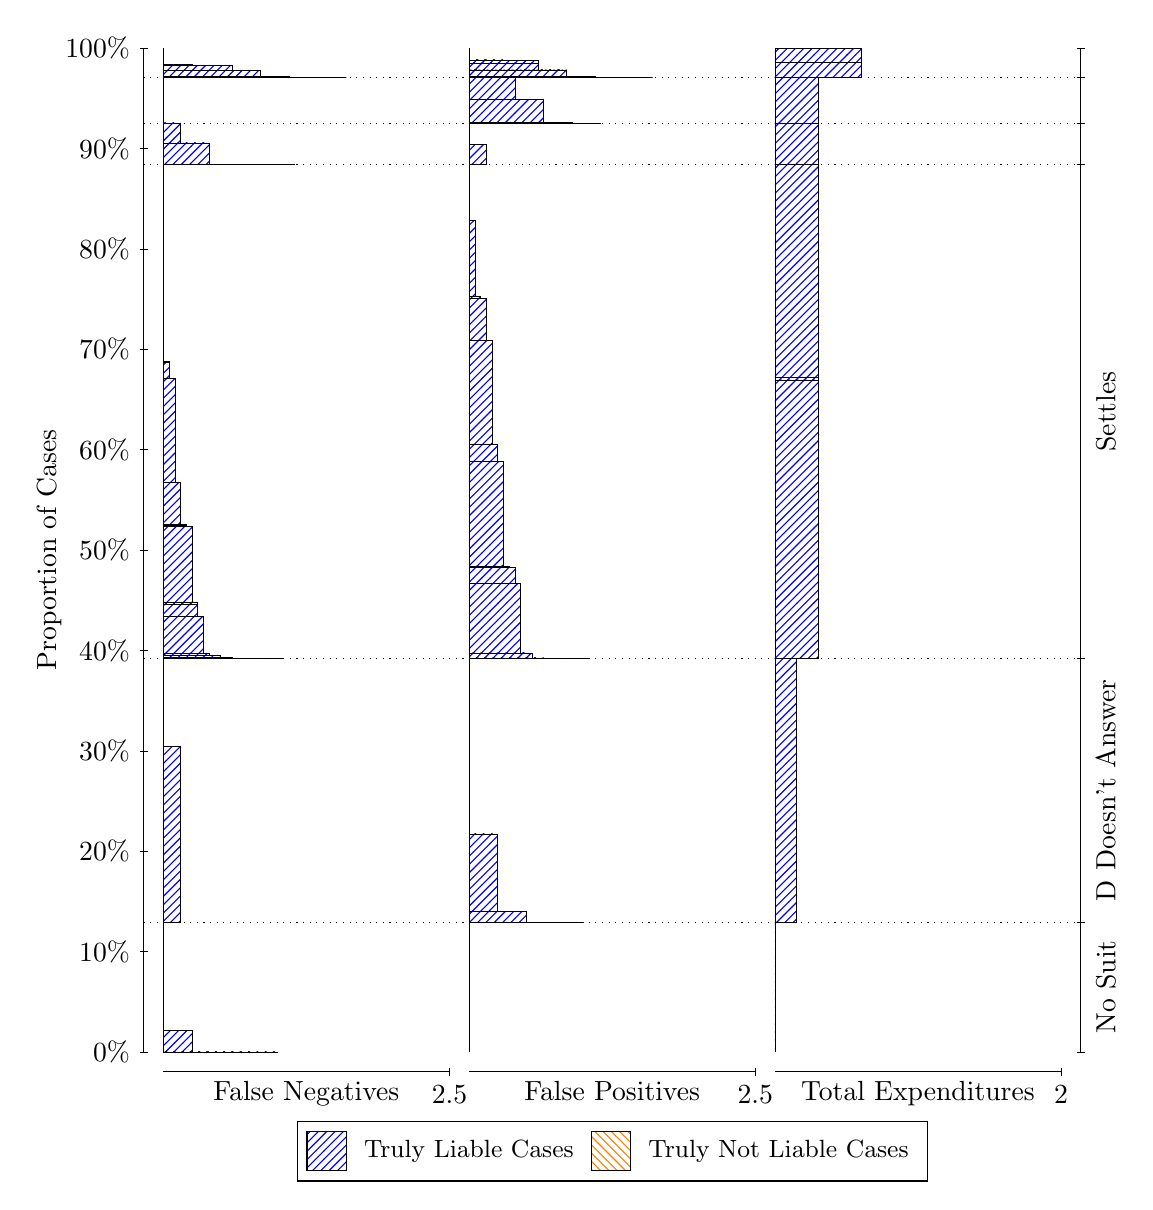
\begin{tikzpicture}
\draw[black, very thin] (1.5,1.75) -- (1.5,14.5);
\node[rotate=90, text=black, anchor=center] at (0.3, 8.125) {Proportion of Cases};
\draw[black, very thin] (1.45,1.75) -- (1.55,1.75);
\node[text=black, anchor=east] at (1.45, 1.75) {0\%};
\draw[black, very thin] (1.45,3.025) -- (1.55,3.025);
\node[text=black, anchor=east] at (1.45, 3.025) {10\%};
\draw[black, very thin] (1.45,4.3) -- (1.55,4.3);
\node[text=black, anchor=east] at (1.45, 4.3) {20\%};
\draw[black, very thin] (1.45,5.575) -- (1.55,5.575);
\node[text=black, anchor=east] at (1.45, 5.575) {30\%};
\draw[black, very thin] (1.45,6.85) -- (1.55,6.85);
\node[text=black, anchor=east] at (1.45, 6.85) {40\%};
\draw[black, very thin] (1.45,8.125) -- (1.55,8.125);
\node[text=black, anchor=east] at (1.45, 8.125) {50\%};
\draw[black, very thin] (1.45,9.4) -- (1.55,9.4);
\node[text=black, anchor=east] at (1.45, 9.4) {60\%};
\draw[black, very thin] (1.45,10.675) -- (1.55,10.675);
\node[text=black, anchor=east] at (1.45, 10.675) {70\%};
\draw[black, very thin] (1.45,11.95) -- (1.55,11.95);
\node[text=black, anchor=east] at (1.45, 11.95) {80\%};
\draw[black, very thin] (1.45,13.225) -- (1.55,13.225);
\node[text=black, anchor=east] at (1.45, 13.225) {90\%};
\draw[black, very thin] (1.45,14.5) -- (1.55,14.5);
\node[text=black, anchor=east] at (1.45, 14.5) {100\%};

\draw[black, very thin] (13.4,1.75) -- (13.4,14.5);
\draw[black, very thin] (13.35,1.75) -- (13.45,1.75);
\node[anchor=west] at (13.35, 1.75) {};
\draw[black, very thin] (13.35,3.3995) -- (13.45,3.3995);
\node[anchor=west] at (13.35, 3.3995) {};
\draw[black, very thin] (13.35,6.7482) -- (13.45,6.7482);
\node[anchor=west] at (13.35, 6.7482) {};
\draw[black, very thin] (13.35,13.022) -- (13.45,13.022);
\node[anchor=west] at (13.35, 13.022) {};
\draw[black, very thin] (13.35,13.547) -- (13.45,13.547);
\node[anchor=west] at (13.35, 13.547) {};
\draw[black, very thin] (13.35,14.131) -- (13.45,14.131);
\node[anchor=west] at (13.35, 14.131) {};
\draw[black, very thin] (13.35,14.5) -- (13.45,14.5);
\node[anchor=west] at (13.35, 14.5) {};

\draw[black, very thin, pattern color=blue, pattern=north east lines] (1.75,1.75) rectangle (3.2033,1.75);
\draw[black, very thin, pattern color=blue, pattern=north east lines] (1.75,1.75) rectangle (2.84,1.75);
\draw[black, very thin, pattern color=blue, pattern=north east lines] (1.75,1.75) rectangle (2.4767,1.7523);
\draw[black, very thin, pattern color=blue, pattern=north east lines] (1.75,1.7523) rectangle (2.1133,2.0201);
\draw[black, very thin, pattern color=orange, pattern=north west lines] (1.75,2.0201) rectangle (1.75,2.0201);
\draw[black, very thin, pattern color=blue, pattern=north east lines] (1.75,2.0201) rectangle (1.75,3.3995);
\draw[black, very thin, pattern color=blue, pattern=north east lines] (1.75,3.3995) rectangle (1.968,5.6275);
\draw[black, very thin, pattern color=orange, pattern=north west lines] (1.75,5.6275) rectangle (1.75,5.6275);
\draw[black, very thin, pattern color=blue, pattern=north east lines] (1.75,5.6275) rectangle (1.75,6.7482);
\draw[black, very thin, pattern color=blue, pattern=north east lines] (1.75,6.7482) rectangle (3.276,6.7482);
\draw[black, very thin, pattern color=blue, pattern=north east lines] (1.75,6.7482) rectangle (3.1307,6.7482);
\draw[black, very thin, pattern color=blue, pattern=north east lines] (1.75,6.7482) rectangle (2.9853,6.7482);
\draw[black, very thin, pattern color=blue, pattern=north east lines] (1.75,6.7482) rectangle (2.9127,6.7482);
\draw[black, very thin, pattern color=blue, pattern=north east lines] (1.75,6.7482) rectangle (2.84,6.7482);
\draw[black, very thin, pattern color=blue, pattern=north east lines] (1.75,6.7482) rectangle (2.7673,6.7482);
\draw[black, very thin, pattern color=blue, pattern=north east lines] (1.75,6.7482) rectangle (2.6947,6.7482);
\draw[black, very thin, pattern color=blue, pattern=north east lines] (1.75,6.7482) rectangle (2.622,6.7597);
\draw[black, very thin, pattern color=blue, pattern=north east lines] (1.75,6.7597) rectangle (2.5493,6.7606);
\draw[black, very thin, pattern color=blue, pattern=north east lines] (1.75,6.7606) rectangle (2.4767,6.7857);
\draw[black, very thin, pattern color=blue, pattern=north east lines] (1.75,6.7857) rectangle (2.404,6.7857);
\draw[black, very thin, pattern color=blue, pattern=north east lines] (1.75,6.7857) rectangle (2.404,6.7861);
\draw[black, very thin, pattern color=blue, pattern=north east lines] (1.75,6.7861) rectangle (2.3313,6.8098);
\draw[black, very thin, pattern color=blue, pattern=north east lines] (1.75,6.8098) rectangle (2.2587,7.2842);
\draw[black, very thin, pattern color=blue, pattern=north east lines] (1.75,7.2842) rectangle (2.186,7.4409);
\draw[black, very thin, pattern color=blue, pattern=north east lines] (1.75,7.4409) rectangle (2.186,7.4598);
\draw[black, very thin, pattern color=blue, pattern=north east lines] (1.75,7.4598) rectangle (2.1133,8.4234);
\draw[black, very thin, pattern color=blue, pattern=north east lines] (1.75,8.4234) rectangle (2.0407,8.4438);
\draw[black, very thin, pattern color=blue, pattern=north east lines] (1.75,8.4438) rectangle (2.0407,8.4521);
\draw[black, very thin, pattern color=blue, pattern=north east lines] (1.75,8.4521) rectangle (1.968,8.9852);
\draw[black, very thin, pattern color=blue, pattern=north east lines] (1.75,8.9852) rectangle (1.8953,10.308);
\draw[black, very thin, pattern color=blue, pattern=north east lines] (1.75,10.308) rectangle (1.8227,10.505);
\draw[black, very thin, pattern color=blue, pattern=north east lines] (1.75,10.505) rectangle (1.8227,10.52);
\draw[black, very thin, pattern color=orange, pattern=north west lines] (1.75,10.52) rectangle (1.75,10.52);
\draw[black, very thin, pattern color=blue, pattern=north east lines] (1.75,10.52) rectangle (1.75,13.022);
\draw[black, very thin, pattern color=blue, pattern=north east lines] (1.75,13.022) rectangle (3.4213,13.022);
\draw[black, very thin, pattern color=blue, pattern=north east lines] (1.75,13.022) rectangle (3.058,13.022);
\draw[black, very thin, pattern color=blue, pattern=north east lines] (1.75,13.022) rectangle (2.6947,13.027);
\draw[black, very thin, pattern color=blue, pattern=north east lines] (1.75,13.027) rectangle (2.3313,13.296);
\draw[black, very thin, pattern color=blue, pattern=north east lines] (1.75,13.296) rectangle (1.968,13.547);
\draw[black, very thin, pattern color=orange, pattern=north west lines] (1.75,13.547) rectangle (1.75,13.547);
\draw[black, very thin, pattern color=blue, pattern=north east lines] (1.75,13.547) rectangle (1.968,13.55);
\draw[black, very thin, pattern color=orange, pattern=north west lines] (1.75,13.55) rectangle (1.75,13.55);
\draw[black, very thin, pattern color=blue, pattern=north east lines] (1.75,13.55) rectangle (1.75,14.131);
\draw[black, very thin, pattern color=blue, pattern=north east lines] (1.75,14.131) rectangle (4.0753,14.131);
\draw[black, very thin, pattern color=blue, pattern=north east lines] (1.75,14.131) rectangle (3.712,14.131);
\draw[black, very thin, pattern color=blue, pattern=north east lines] (1.75,14.131) rectangle (3.3487,14.137);
\draw[black, very thin, pattern color=blue, pattern=north east lines] (1.75,14.137) rectangle (2.9853,14.216);
\draw[black, very thin, pattern color=blue, pattern=north east lines] (1.75,14.216) rectangle (2.84,14.216);
\draw[black, very thin, pattern color=blue, pattern=north east lines] (1.75,14.216) rectangle (2.622,14.28);
\draw[black, very thin, pattern color=blue, pattern=north east lines] (1.75,14.28) rectangle (2.4767,14.28);
\draw[black, very thin, pattern color=blue, pattern=north east lines] (1.75,14.28) rectangle (2.2587,14.281);
\draw[black, very thin, pattern color=blue, pattern=north east lines] (1.75,14.281) rectangle (2.1133,14.288);
\draw[black, very thin, pattern color=blue, pattern=north east lines] (1.75,14.288) rectangle (1.8953,14.288);
\draw[black, very thin, pattern color=orange, pattern=north west lines] (1.75,14.288) rectangle (1.75,14.288);
\draw[black, very thin, pattern color=blue, pattern=north east lines] (1.75,14.288) rectangle (1.75,14.5);
\draw[black, very thin, pattern color=orange, pattern=north west lines] (5.6333,1.75) rectangle (5.6333,1.75);
\draw[black, very thin, pattern color=blue, pattern=north east lines] (5.6333,1.75) rectangle (5.6333,3.3995);
\draw[black, very thin, pattern color=orange, pattern=north west lines] (5.6333,3.3995) rectangle (7.0867,3.3995);
\draw[black, very thin, pattern color=blue, pattern=north east lines] (5.6333,3.3995) rectangle (7.0867,3.3995);
\draw[black, very thin, pattern color=blue, pattern=north east lines] (5.6333,3.3995) rectangle (6.7233,3.4005);
\draw[black, very thin, pattern color=blue, pattern=north east lines] (5.6333,3.4005) rectangle (6.36,3.5375);
\draw[black, very thin, pattern color=blue, pattern=north east lines] (5.6333,3.5375) rectangle (5.9967,4.5202);
\draw[black, very thin, pattern color=blue, pattern=north east lines] (5.6333,4.5202) rectangle (5.6333,6.7482);
\draw[black, very thin, pattern color=orange, pattern=north west lines] (5.6333,6.7482) rectangle (7.1593,6.7482);
\draw[black, very thin, pattern color=blue, pattern=north east lines] (5.6333,6.7482) rectangle (7.1593,6.7482);
\draw[black, very thin, pattern color=orange, pattern=north west lines] (5.6333,6.7482) rectangle (6.8687,6.7482);
\draw[black, very thin, pattern color=blue, pattern=north east lines] (5.6333,6.7482) rectangle (6.8687,6.7482);
\draw[black, very thin, pattern color=blue, pattern=north east lines] (5.6333,6.7482) rectangle (6.796,6.7482);
\draw[black, very thin, pattern color=orange, pattern=north west lines] (5.6333,6.7482) rectangle (6.7233,6.7482);
\draw[black, very thin, pattern color=blue, pattern=north east lines] (5.6333,6.7482) rectangle (6.7233,6.7482);
\draw[black, very thin, pattern color=orange, pattern=north west lines] (5.6333,6.7482) rectangle (6.578,6.7482);
\draw[black, very thin, pattern color=blue, pattern=north east lines] (5.6333,6.7482) rectangle (6.578,6.7552);
\draw[black, very thin, pattern color=blue, pattern=north east lines] (5.6333,6.7552) rectangle (6.5053,6.7552);
\draw[black, very thin, pattern color=orange, pattern=north west lines] (5.6333,6.7552) rectangle (6.4327,6.7552);
\draw[black, very thin, pattern color=blue, pattern=north east lines] (5.6333,6.7552) rectangle (6.4327,6.816);
\draw[black, very thin, pattern color=blue, pattern=north east lines] (5.6333,6.816) rectangle (6.36,6.818);
\draw[black, very thin, pattern color=orange, pattern=north west lines] (5.6333,6.818) rectangle (6.2873,6.818);
\draw[black, very thin, pattern color=blue, pattern=north east lines] (5.6333,6.818) rectangle (6.2873,7.7019);
\draw[black, very thin, pattern color=blue, pattern=north east lines] (5.6333,7.7019) rectangle (6.2147,7.9029);
\draw[black, very thin, pattern color=orange, pattern=north west lines] (5.6333,7.9029) rectangle (6.142,7.9029);
\draw[black, very thin, pattern color=blue, pattern=north east lines] (5.6333,7.9029) rectangle (6.142,7.9239);
\draw[black, very thin, pattern color=blue, pattern=north east lines] (5.6333,7.9239) rectangle (6.0693,9.2499);
\draw[black, very thin, pattern color=orange, pattern=north west lines] (5.6333,9.2499) rectangle (5.9967,9.2499);
\draw[black, very thin, pattern color=blue, pattern=north east lines] (5.6333,9.2499) rectangle (5.9967,9.4619);
\draw[black, very thin, pattern color=blue, pattern=north east lines] (5.6333,9.4619) rectangle (5.924,10.785);
\draw[black, very thin, pattern color=blue, pattern=north east lines] (5.6333,10.785) rectangle (5.8513,11.318);
\draw[black, very thin, pattern color=blue, pattern=north east lines] (5.6333,11.318) rectangle (5.7787,11.347);
\draw[black, very thin, pattern color=blue, pattern=north east lines] (5.6333,11.347) rectangle (5.706,12.31);
\draw[black, very thin, pattern color=blue, pattern=north east lines] (5.6333,12.31) rectangle (5.6333,13.022);
\draw[black, very thin, pattern color=orange, pattern=north west lines] (5.6333,13.022) rectangle (5.8513,13.022);
\draw[black, very thin, pattern color=blue, pattern=north east lines] (5.6333,13.022) rectangle (5.8513,13.273);
\draw[black, very thin, pattern color=blue, pattern=north east lines] (5.6333,13.273) rectangle (5.6333,13.547);
\draw[black, very thin, pattern color=orange, pattern=north west lines] (5.6333,13.547) rectangle (7.3047,13.547);
\draw[black, very thin, pattern color=blue, pattern=north east lines] (5.6333,13.547) rectangle (7.3047,13.547);
\draw[black, very thin, pattern color=blue, pattern=north east lines] (5.6333,13.547) rectangle (6.9413,13.551);
\draw[black, very thin, pattern color=blue, pattern=north east lines] (5.6333,13.551) rectangle (6.578,13.846);
\draw[black, very thin, pattern color=blue, pattern=north east lines] (5.6333,13.846) rectangle (6.2147,14.128);
\draw[black, very thin, pattern color=blue, pattern=north east lines] (5.6333,14.128) rectangle (5.8513,14.131);
\draw[black, very thin, pattern color=orange, pattern=north west lines] (5.6333,14.131) rectangle (7.9587,14.131);
\draw[black, very thin, pattern color=blue, pattern=north east lines] (5.6333,14.131) rectangle (7.9587,14.131);
\draw[black, very thin, pattern color=orange, pattern=north west lines] (5.6333,14.131) rectangle (7.5953,14.131);
\draw[black, very thin, pattern color=blue, pattern=north east lines] (5.6333,14.131) rectangle (7.5953,14.131);
\draw[black, very thin, pattern color=orange, pattern=north west lines] (5.6333,14.131) rectangle (7.232,14.131);
\draw[black, very thin, pattern color=blue, pattern=north east lines] (5.6333,14.131) rectangle (7.232,14.138);
\draw[black, very thin, pattern color=blue, pattern=north east lines] (5.6333,14.138) rectangle (6.8687,14.222);
\draw[black, very thin, pattern color=orange, pattern=north west lines] (5.6333,14.222) rectangle (6.8687,14.222);
\draw[black, very thin, pattern color=blue, pattern=north east lines] (5.6333,14.222) rectangle (6.8687,14.223);
\draw[black, very thin, pattern color=blue, pattern=north east lines] (5.6333,14.223) rectangle (6.5053,14.312);
\draw[black, very thin, pattern color=blue, pattern=north east lines] (5.6333,14.312) rectangle (6.5053,14.343);
\draw[black, very thin, pattern color=orange, pattern=north west lines] (5.6333,14.343) rectangle (6.36,14.343);
\draw[black, very thin, pattern color=blue, pattern=north east lines] (5.6333,14.343) rectangle (6.36,14.343);
\draw[black, very thin, pattern color=blue, pattern=north east lines] (5.6333,14.343) rectangle (6.142,14.344);
\draw[black, very thin, pattern color=blue, pattern=north east lines] (5.6333,14.344) rectangle (6.142,14.349);
\draw[black, very thin, pattern color=orange, pattern=north west lines] (5.6333,14.349) rectangle (5.9967,14.349);
\draw[black, very thin, pattern color=blue, pattern=north east lines] (5.6333,14.349) rectangle (5.9967,14.35);
\draw[black, very thin, pattern color=blue, pattern=north east lines] (5.6333,14.35) rectangle (5.7787,14.35);
\draw[black, very thin, pattern color=blue, pattern=north east lines] (5.6333,14.35) rectangle (5.7787,14.35);
\draw[black, very thin, pattern color=orange, pattern=north west lines] (5.6333,14.35) rectangle (5.6333,14.35);
\draw[black, very thin, pattern color=blue, pattern=north east lines] (5.6333,14.35) rectangle (5.6333,14.5);
\draw[black, very thin, pattern color=orange, pattern=north west lines] (9.5167,1.75) rectangle (9.5167,1.75);
\draw[black, very thin, pattern color=blue, pattern=north east lines] (9.5167,1.75) rectangle (9.5167,3.3995);
\draw[black, very thin, pattern color=orange, pattern=north west lines] (9.5167,3.3995) rectangle (9.7892,3.3995);
\draw[black, very thin, pattern color=blue, pattern=north east lines] (9.5167,3.3995) rectangle (9.7892,6.7482);
\draw[black, very thin, pattern color=orange, pattern=north west lines] (9.5167,6.7482) rectangle (10.062,6.7482);
\draw[black, very thin, pattern color=blue, pattern=north east lines] (9.5167,6.7482) rectangle (10.062,10.285);
\draw[black, very thin, pattern color=orange, pattern=north west lines] (9.5167,10.285) rectangle (10.062,10.285);
\draw[black, very thin, pattern color=blue, pattern=north east lines] (9.5167,10.285) rectangle (10.062,10.32);
\draw[black, very thin, pattern color=orange, pattern=north west lines] (9.5167,10.32) rectangle (10.062,10.32);
\draw[black, very thin, pattern color=blue, pattern=north east lines] (9.5167,10.32) rectangle (10.062,13.022);
\draw[black, very thin, pattern color=orange, pattern=north west lines] (9.5167,13.022) rectangle (10.062,13.022);
\draw[black, very thin, pattern color=blue, pattern=north east lines] (9.5167,13.022) rectangle (10.062,13.547);
\draw[black, very thin, pattern color=orange, pattern=north west lines] (9.5167,13.547) rectangle (10.062,13.547);
\draw[black, very thin, pattern color=blue, pattern=north east lines] (9.5167,13.547) rectangle (10.062,14.131);
\draw[black, very thin, pattern color=orange, pattern=north west lines] (9.5167,14.131) rectangle (10.607,14.131);
\draw[black, very thin, pattern color=blue, pattern=north east lines] (9.5167,14.131) rectangle (10.607,14.313);
\draw[black, very thin, pattern color=orange, pattern=north west lines] (9.5167,14.313) rectangle (10.607,14.313);
\draw[black, very thin, pattern color=blue, pattern=north east lines] (9.5167,14.313) rectangle (10.607,14.5);
\draw[black, dotted] (1.5,3.3995) -- (13.4,3.3995);
\draw[black, dotted] (1.5,6.7482) -- (13.4,6.7482);
\draw[black, dotted] (1.5,13.022) -- (13.4,13.022);
\draw[black, dotted] (1.5,13.547) -- (13.4,13.547);
\draw[black, dotted] (1.5,14.131) -- (13.4,14.131);
\draw[black, very thin] (1.75,1.5) -- (5.3833,1.5);
\node[text=black, anchor=north] at (3.5667, 1.5) {False Negatives};
\draw[black, very thin] (5.3833,1.45) -- (5.3833,1.55);
\node[text=black, anchor=north] at (5.3833, 1.45) {2.5};

\draw[black, very thin] (5.6333,1.5) -- (9.2667,1.5);
\node[text=black, anchor=north] at (7.45, 1.5) {False Positives};
\draw[black, very thin] (9.2667,1.45) -- (9.2667,1.55);
\node[text=black, anchor=north] at (9.2667, 1.45) {2.5};

\draw[black, very thin] (9.5167,1.5) -- (13.15,1.5);
\node[text=black, anchor=north] at (11.333, 1.5) {Total Expenditures};
\draw[black, very thin] (13.15,1.45) -- (13.15,1.55);
\node[text=black, anchor=north] at (13.15, 1.45) {2};

\node[text=black, centered, rotate=90] at (13.72, 2.5748) {No Suit};
\node[text=black, centered, rotate=90] at (13.72, 5.0739) {D Doesn't Answer};
\node[text=black, centered, rotate=90] at (13.72, 9.8851) {Settles};




\draw (7.449999999999999,1.5) node[draw=none] (baseCoordinate) {};
\begin{scope}[align=center]
        \matrix[scale=0.5, draw=black, below=0.5cm of baseCoordinate, nodes={draw}, column sep=0.1cm]{
            \node[rectangle, draw, minimum width=0.5cm, minimum height=0.5cm, pattern color=blue, pattern=north east lines] {}; &
            \node[draw=none, font=\small, text=black] (B) {Truly Liable Cases}; &
            \node[rectangle, draw, minimum width=0.5cm, minimum height=0.5cm, pattern color=orange, pattern=north west lines] {}; &
            \node[draw=none, font=\small, text=black] (B) {Truly Not Liable Cases}; \\
            };
\end{scope}

\end{tikzpicture}
\end{document}